\documentclass[a4paper,12pt,DIV=calc]{scrartcl}

% Character Encoding
\usepackage[utf8]{inputenc}
\usepackage[T1]{fontenc}

% Math Typesetting
\usepackage{amsmath}

% URLs
\usepackage{url}
\usepackage[pdfusetitle,hidelinks]{hyperref}

% Various Typesetting Packages
\usepackage{microtype}
\usepackage[british]{babel}

% Tikz
\usepackage{tikz}
\usetikzlibrary{positioning}

% Figure frames
\usepackage{mdframed}

% Code references (command is mainly used so I can keep track of them easily)
%TC:macro \coderef [ignore,ignore,ignore]
\newcommand{\coderef}[3]{\emph{(#1, #2, #3)}}

\begin{document}
% Title
\title{EMBS WSN MAC Layer Protocol Report}
\author{James Cowgill}
\date{27th November 2015}
\maketitle

%Report entry 1:
% - Design + Implementation Decisions
%   - Synchronizing to multiple sinks
%   + Handling of sinks with n = 1
% - References of the form (class name, method name, line numbers)
%   - For every decision
% - Max 400 words, does not include references and figures
% + "well illustrated"
%
%Report entry 2:
% - Design + Implementation Decisions
%   - Synchronizing to multiple sinks
%   - Design decisions related to energy efficiency
% - References as above
% - Max 500 words as above

\section{Exercise 1 - Ptolemy II}
\begin{figure}[ht]
  \centering
  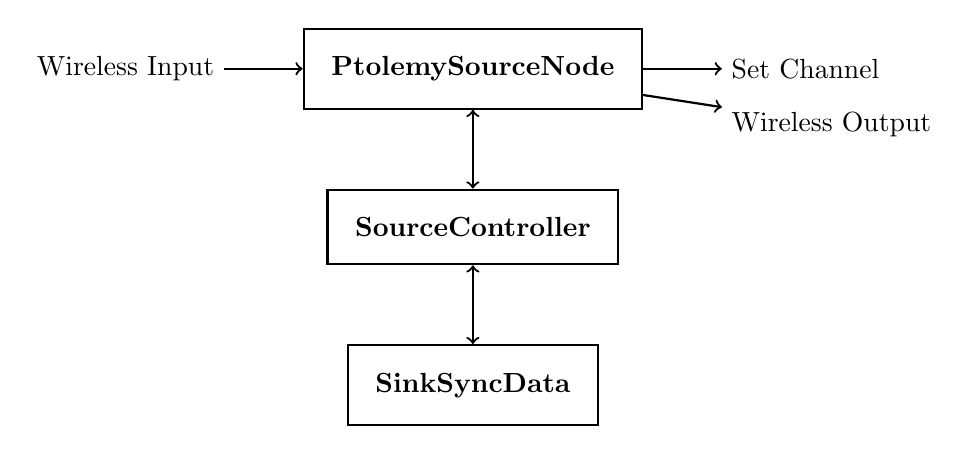
\begin{tikzpicture}[
     class/.style={draw, rectangle, thick, align=center, inner sep=1em,
       font=\bfseries},
     port/.style={},
     arrow/.style={thick}]

    \node(SourceNode)       [class] {PtolemySourceNode};
    \node(SourceController) [class,below=of SourceNode] {SourceController}
      edge [<->,arrow] (SourceNode);
    \node(SinkSyncData)     [class,below=of SourceController] {SinkSyncData}
      edge [<->,arrow] (SourceController);

    \node(inWifi)           [port,left=of SourceNode] {Wireless Input}
      edge [->,arrow] (SourceNode);
    \node(setChannel)       [port,right=of SourceNode] {Set Channel}
      edge [<-,arrow] (SourceNode);
    \node(outWifi)          [port,below=2em of setChannel.west,anchor=west]
      {Wireless Output} edge [<-,arrow] (SourceNode);
  \end{tikzpicture}
  \caption{Exercise 1 Block Diagram}
\end{figure}

The design for the system I implemented for Exercise 1 is split into 3 classes to
try and modularize the code and separate the different tasks. Each is described
separately in this report.

\subsection{SinkSyncData}
The SinkSyncData class contains the main algorithm which calculates the $n$ and
$t$ values for each sink. It also contains the code to calculate the time to
send the next packet to each sink.

From the initial problem, it is possible to derive a function giving the exact
time each beacon frame will be received by the source.

\begin{figure}[ht]
  \begin{mdframed}
  \centering
    \begin{equation*}
      f(s, n, t, i, b) = ((11 + n)i - (b - 1)t + s
    \end{equation*}
    \begin{description}
      \itemsep0em
      \item[$s$] Absolute start time
      \item[$n$] Value of n from the protocol, number of beacons to be sent
      \item[$t$] Value of t from the protocol, time between beacons
      \item[$i$] Integer iteration number
      \item[$b$] Integer beacon number within this iteration (1 \dots $n$)
    \end{description}
  \end{mdframed}
  \caption{Function giving the exact time of each beacon}
\end{figure}

This function gives the absolute time a beacon occurs, but to eliminate the
value of $s$ we will subtract the times of two beacons received from a
particular sink. The function giving the time between beacons simplifies to:
\begin{align*}
  \Delta t &= f(s, n, t, i_2, b_2) - f(s, n, t, i_1, b_1) \\
           &= ((11 + n)(i_2 - i_1) - b_2 + b_1)t
\end{align*}

This is then used within the receiveBeacon function \coderef{SinkSyncData}
{receiveBeacon}{78-150} to calculate good values for $n$ and $t$. By recording
the time and $n$ value of the previous beacon, we will always know the values
of $\Delta t$, $b_1$ and $b_2$. The main part of the
algorithm calculates $t$ exactly when it knows about two adjacent beacons from
the same iteration. It can then calculate $n$ exactly by measuring the duration
of the sleep period.

In the case where $n = 1$, the easiest way of calculating $t$ using two adjacent
beacons is not possible, so the only way is to measure beacons from different
iterations and use the time taken in the sleep period. The algorithm does this
by guessing at an iteration length of one. This usually works, but can give the
wrong results if some beacons are skipped over.

\subsection{SourceController}
This class coordinates multiple sinks and stores references to the SinkSyncData
objects for each sink.  When beacons are received, they're forwarded to the
relevant sink object and the channel might be changed
\coderef{SourceController}{receiveBeacon}{145-167}.

All decisions to change the channel receiving beacons are controlled by this
class \coderef{SourceController}{changeChannel}{170-195}. With a few exceptions
that apply after beacons have been received, this happens every second. This is
done to avoid wasting time staying on one channel when no useful information
can be gathered for some time. The main disadvantage is that it's difficult to
be certain about the values for $n$ and $t$ in the $n = 1$ case when doing this.

One exception to the channel change time limit is that a channel will get some
extra time if a beacon was recently received, and another is likely to be
received very shortly. This should increase the chances of a good value of $t$
being calculated by obtaining beacons from the same protocol iteration.

\subsection{PtolemySourceNode}
This class contains the Ptolemy specific code. All the interesting parts of the
model are implemented in Java here (only connections to wireless ports are
outside the class).

When the actor is fired, any beacons received are forwarded to the
SourceController instance \coderef{PtolemySourceNode}{fire}{131-146} and any
packets to be sent and channel changes are handled. In Ptolemy, changing the
channel can happen at any time, but it's not possible to send two packets to
different channels within the same fire event. To workaround this, whenever a
packet is sent, the actor fires itself so it can handle any subsequent packets
\coderef{PtolemySourceNode}{sendPendingPacket}{106-112}.

Timer events are also handled by the actor firing itself, but since the time
until the actor wakes up could decrease (e.g. if we receive an $n = 1$ beacon,
we might need to transmit a packet in a short time), the time is recorded so
that any spurious timer events can be dropped.

\section{Exercise 2 - Mote Runner}
For the second exercise, I chose to reuse the back end parts of the code I wrote
for Ptolemy. This was enabled since both Ptolemy and Mote Runner can be
programmed in Java. Reusing the code meant I had to write much less code in
total, and allows simulation in Ptolemy of the actual code in the final
implementation. Since the code for Ptolemy was designed to take into account the
loss of random beacons (since SourceController can change the channel at will),
the code should still work in the real world where beacons can be lost for
various reasons during normal operation. The difficult case of $n = 1$ also does
not apply here. As the code is being reused, all the policy decisions relating
to the calculation of $n$ and $t$ values, and the handling of multiple sinks are
the same as the previous exercise.

The implementation for exercise 2 revolves around the
handleControllerStateChange method
\coderef{MoteSourceNode}{handleControllerStateRef}{194-252}. This method is
called after each type of event has been processed to try and update the state
of the radio to what the SourceController class wants. Most actions (such as the
scheduling of a timer event, starting the receiver and transmitting packets) are
initiated here.

Unlike the Ptolemy model, it is not possible to change the channel of the Mote
Runner radio while receiving or transmitting. To workaround this, the state of
the radio is recorded in two variables (txOn and rxOn), and the tryChangeChannel
method \coderef{MoteSourceNode}{tryChangeChannel}{261-279} will only attempt to
change channels if these variables are false. Otherwise it will wait for the
radio to finish, and the call to tryChangeChannel will be retried later.

Since the assignment did not place any emphasis on energy efficiency, I mostly
ignored it and tried instead to get the packet transmissions as accurate as
possible. However, once the source node has synced with all the sink nodes, it
will turn the radio off to save energy since no more information needs to be
gathered.

\end{document}
